\documentclass[a4paper,12pt]{article}


\usepackage[T1]{fontenc}
\usepackage[utf8]{inputenc}
\usepackage[frenchb]{babel}


\usepackage{graphicx}
\usepackage{xspace}


\title{Compte rendu de travaux pratiques\\ \small ou un meilleur titre}
\author{Vincent Denechaud, Olivier Maillet, Alice Odier, Félix Tora}
\date{Vendredi 24 janvier 2014}

\newcommand\ett{Everhart et Thornley\xspace}




\begin{document}

\maketitle

La microscopie électronique est une des techniques importantes de caractérisation d'échantillon. En effet, elle permet d'avoir accès à un grand nombre d'information. Ce TP est une introduction à l'utilisation du MEB, il permet de mesurer l'ampleur des possibilités de ce type de microscopie et de comprendre les raisonnements permettant d'interpréter les clichés obtenus. C'est pour cela que l'on commencera par introduire les différents électrons mis en jeu et leurs détecteurs associés, pour ensuite s'intéresser aux clichés effectués durant la séance et à l'utilisation de photons X dans l'enceinte du MEB pour compléter les informations disponibles.


\section{Rappel des différentes sources électroniques et leur détection}


\subsection{Les différentes sources électroniques du MEB}

Des électrons sont accélérés depuis la cathode vers l'échantillon que l'on souhaite étudier. Du fait de leur énergie cinétique, les électrons pénètrent dans la matière de l'échantillon en formant ce que l'on appelle une poire d'intéraction (figure \ref{fig:poire_int}).

\begin{figure}
\centering
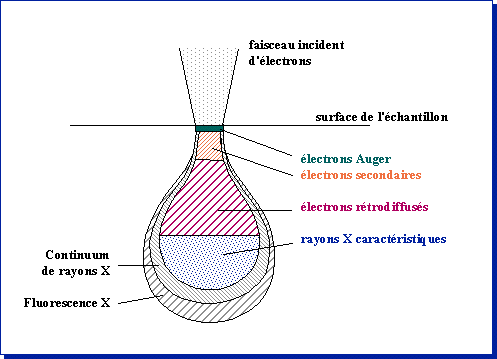
\includegraphics[width = 0.8 \textwidth]{images/poire_int.png}
\caption{Poire d'interaction : on distingue les différents type de rayonnements issus de l'interaction entre le faisceau électronique incident et l'échantillon.}
\label{fig:poire_int}
\end{figure}


En réponse à cette excitation, la matière revient à l'équilibre en émettant du rayonnement X ainsi que des électrons, 
de sorte que le cortège électronique des atomes composant l'échantillon possède une configuration d'équilibre énergétique. 
On peut classer les émissions électroniques selon différentes catégories.

\subsubsection*{Électrons rétro-diffusés}
Lorsque les électrons viennent interagir avec l'échantillon, ils sont, pour la plupart, rétro-diffusés de manière élastique.
Autrement dit, ces électrons interagissent avec les noyaux des atomes de l'échantillon de sorte à conserver leur énergie cinétique.
Ainsi, ces électrons ont une grande profondeur d'échappée et un grand libre parcours moyen dans l'échantillon.
De fait, ces électrons sont très sensibles à la composition chimique de l'échantillon, plus particulièrement, 
au numéro atomique Z des atomes constituant l'échantillon.
Les atomes les plus lourds (Z grand) vont ré-émettre plus d'électrons que les atomes plus légers. L'utilisation des électrons rétro-diffusés permet donc d'avoir un contraste chimique sur l'observation de l'échantillon.
Même s'ils ont une grande longueur de pénétration, ces électrons permettent une résolution spatiale (contraste topographique) de Xnm (figure \ref{fig:poire_int}).

\subsubsection*{Électrons secondaires}
En autre des électrons diffusés de manière quasi-élastique, une autre partie de ces derniers est diffusée de manière inélastique par l'échantillon.
Ce sont les électrons dits secondaires. 
Ces électrons cèdent donc très vite leur énergie cinétique et ont un faible libre parcours moyen ainsi qu'une faible profondeur de pénétration dans l'échantillon. 
Néanmoins, étant donné que ces derniers ressortent très vite de l'échantillon, la résolution spatiale obtenue 
après leur détection est bien meilleure (de l'ordre de $5$nm) que celle obtenue avec les électrons rétro-diffusés.
Les électrons secondaires seront donc très utiles pour réaliser un bon contraste topographique.
On notera cependant qu'il y a beaucoup moins d'électrons du type secondaire que rétro-diffusé. 
L'utilisation des électrons secondaires nécessite donc un temps de pose plus long pour réaliser un cliché.

\subsection{Les techniques de détection associées}

\subsubsection*{Détection des électrons rétro-diffusés}

La détection des électrons rétro-diffusés se fait à l'aide d'un (double) détecteur à semi-conducteur 
(qui n'est généralement rien d'autre qu'une jonction Schottky, cf figure \ref{fig:detect_sc}). 

\begin{figure}
\centering
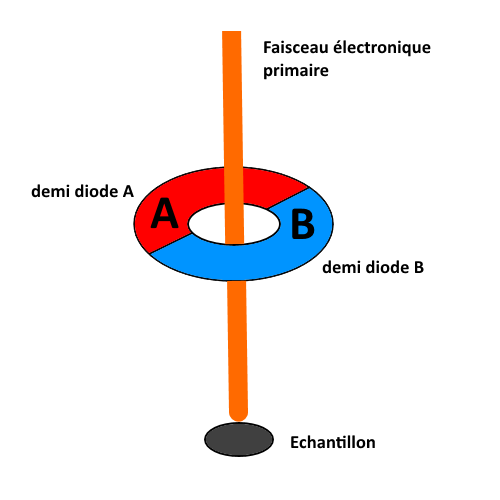
\includegraphics[width = 0.7 \textwidth]{images/detect_sc.png}
\caption{Détecteur à semi-conducteur pour électrons rétro-diffusés. Dans le cas des expériences présentées ici, il s'agit d'un détecteur annulaire positionné dans l'axe du faisceau primaire. On appelle A et B les deux demi-diodes composant le détecteur.}
\label{fig:detect_sc}
\end{figure}


Lorsqu'un électron rétro-diffusé vient frapper la surface semi-conductrice du détecteur, 
et si celui-ci possède une énergie cinétique appropriée,
il y a alors création d'une paire électron-trou dans le semi-conducteur. 
Les porteurs de charge sont alors collectés aux contacts de la jonction, d'où la mesure d'un courant et détection de l'électron rétro-diffusé.

Comme le montre la figure \ref{fig:detect_sc}, le détecteur est composé de deux "demi-diodes".
Un tel découpage permet de mode de fonctionnement.
En effet, il devient possible de séparer le signal donné par le détecteur en deux voies A et B.

Additionner ou soustraire les signaux A et B permet d'obtenir respectivement un contraste de composition de l'échantillon ou bien topographique, comme indiqué figure \ref{fig:detect_sc_contraste}.

\begin{figure}
\centering
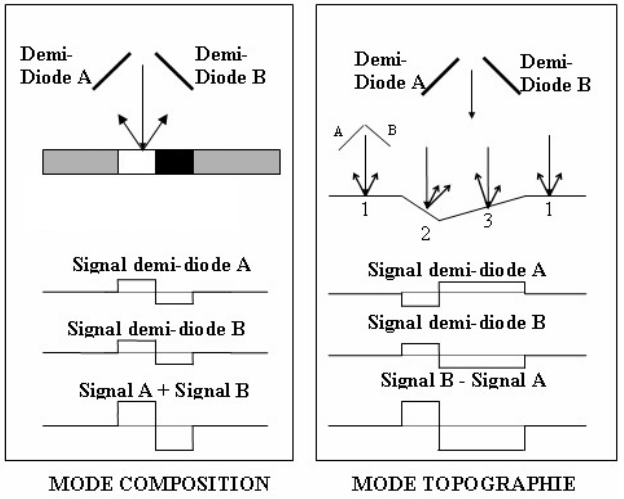
\includegraphics[width = 0.9 \textwidth]{images/detect_sc_contraste.png}
\caption{Contrastes de composition et topographique obtenus en manipulant les voies A et B du détecteur à électrons rétro-diffusés.}
\label{fig:detect_sc_contraste}
\end{figure}







\subsubsection*{Détection des électrons secondaires}

La détection des électrons rétro-diffusés se fait à l'aide du détecteur d'\ett. Il est composé d'une grille, d'un scintillateur et d'un photo-multiplicateur (figure \ref{fig:detect_ett}).

\begin{figure}
\centering
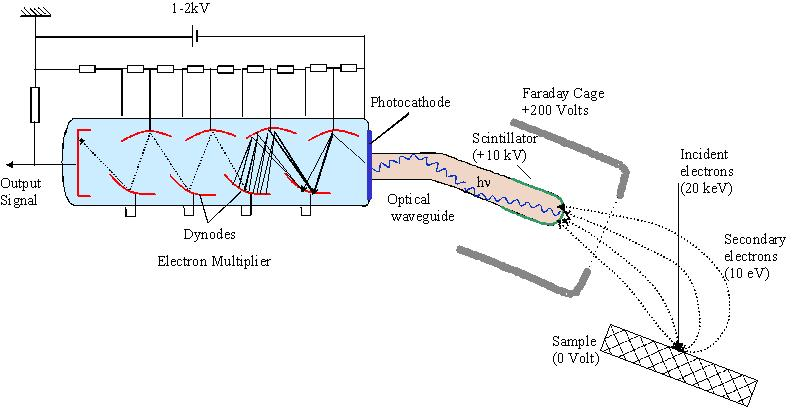
\includegraphics[width = 0.9 \textwidth]{images/detect_ett.png}
\caption{Détecteur d'\ett composé d'un collecteur, d'un scintillateur et d'un photo-multiplicateur.}
\label{fig:detect_ett}
\end{figure}
 
On polarise le collecteur en tension à $+200$ Volts, ce qui a pour rôle d'attirer les électrons secondaires. 
Cette grille joue aussi le rôle de "cage de Faraday", ce qui permet de ne pas attirer des électrons du faisceau incident. 
Les électrons secondaires possédant une faible énergie, ils sont ainsi sélectionnés par rapport aux électrons rétro-diffusés.
Il reste néanmoins les électrons rétro-diffusés avec l'angle solide correspondant à la direction du détecteur d'\ett dont l'on ne peut pas s'affranchir.

Une fois les électrons collectés, ils sont accélérés vers un scintillateur polarisé à $10$kV qui les "transforme" en photons.
Ces photons sont ensuite conduits vers un photo-multiplicateur qui a pour but d'amplifier le signal final obtenu.


Il est possible d'utiliser le détecteur d'\ett  pour détecter les électrons rétro-diffusés.
En effet, en polarisant négativement le collecteur, les électrons secondaires émis à la surface de l'échantillon sont repoussés.
Ainsi, on ne détecte que les électrons rétro-diffusés possédant l'angle solide associé à la position du détecteur d'\ett, dit électrons rétro-diffusés à incidence rasante.
Une telle manipulation permet d'obtenir des informations complémentaires sur le contraste topographique.


\subsection{Grandissement et mise au point}
Dans le MEB, le grandissement n'est pas du aux lentilles comme dans les microscopes optiques traditionnels mais à la taille de la zone de balayage. Plus la zone de balayage est petite plus le grandissement sera grand. Le réglage de la netteté ne se fait donc pas comme en optique en déplaçant les lentilles. Ici c'est le rapport entre la taille du faisceau et la taille de la zone de balayage qui définit la netteté. Pour que l'image soit nette, il faut que la taille du faisceau soit plus petite que le pas de balayage pour éviter tout recouvrement. On cherche donc à focaliser de manière à remplir cette condition et cela se fait en changeant la focale des lentilles. En effet comme ce sont des lentilles électromagnétiques, leur focale peut être changée en modifiant le courant qui les traverse.


C'est le fait que le grandissement ne dépendent pas des lentilles qui permet d'avoir une résolution bien plus grande. Comme la distance de travail est beaucoup plus grande qu'en optique et donc l'angle bien plus petit, on obtient des profondeurs de champs plus importante qu'en microscopie optique. 



\section{Echantillon éponge de Nickel}

L'observation de ce premier échantillon, une éponge de nickel, va nous permettre d'illustrer l'utilisation des différentes techniques présentées précédemment.

\subsection{Détecteur d'\ett}

Utilisant comme technique d'imagerie intiale les électrons secondaires recueillis par le détecteur d'\ett,
on accède à une première observation de l'échantillon présentée figure \ref{fig:ni_es}. Comme déjà évoqué,
cette technique a l'avantage d'offrir une grande profondeur de champ à l'image obtenue contrairement aux microscopies optiques. Cette première technique d'imagerie permet un contraste de profondeur de champ et donc de visualiser spatialement la forme de l'échantillon.

\begin{figure}
\centering
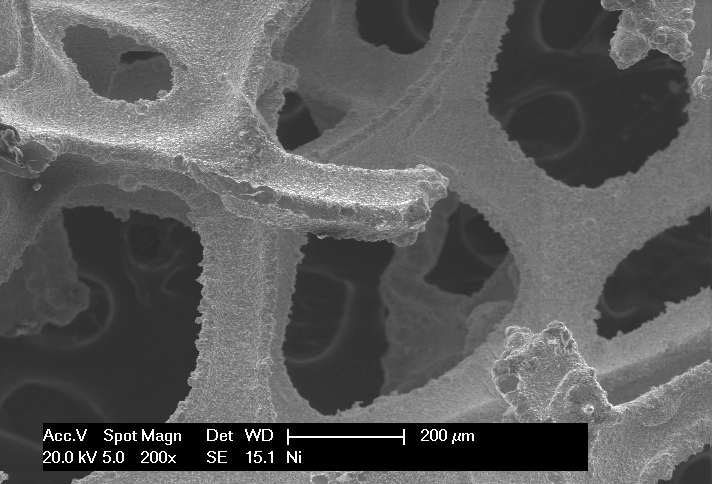
\includegraphics[width = 0.7 \textwidth]{images/ni_es.png}
\caption{Observation de l'éponge de nickel utilisant les électrons secondaires recueillis par le détecteur d'\ett. L'échantillon est ici grossi 200 fois.}
\label{fig:ni_es}
\end{figure}

Le détecteur d'\ett permet aussi de récolter des électrons rétro-diffusés. Ces électrons rétro-diffusés sont
collectés dans un angle solide bien précis, ainsi l'image obtenue à l'aide de cette technique présente une
certaine profondeur de champ mais aussi des effets d'ombre et de lumière. Ces effets sont dus à l'angle
d'incidence des électrons collectés. L'image obtenue à l'aide de cette technique est présentée figure
\ref{fig:ni_er_rasant}.

\begin{figure}
\centering
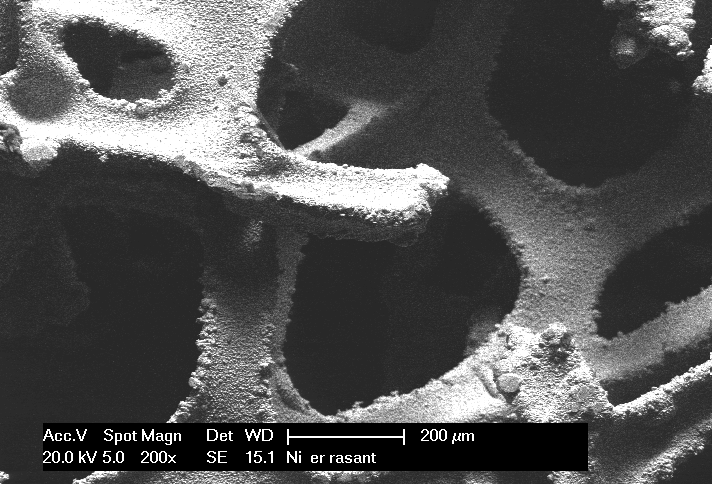
\includegraphics[width = 0.7 \textwidth]{images/ni_er_rasant.png}
\caption{Observation de l'éponge de nickel utilisant les électrons rétro-diffusés recueillis par le détecteur d'\ett. L'échantillon est ici grossi 200 fois.}
\label{fig:ni_er_rasant}
\end{figure}


\subsection{Détecteur à semi-conducteur}

L'utilisation du détecteur à semi-conducteur permet de collecter un grand nombre d'électrons rétro-diffusés
et d'obtenir deux types d'imagerie. L'utilisation du mode $A+B$ permet d'obtenir une image avec un contraste
en composition chimique. L'image de l'éponge de nickel obtenue avec cette technique est présentée à la figure
\ref{fig:ni_er_apb_amb}. Sur cette image on voit que la profondeur de champ du cliché est très faible. Cependant
le contraste en composition chimique permet d'obtenir d'autres informations tout aussi importantes.

On peut voir sur l'échantillon certaines excroissances qui apparaissent plus foncées. Cette image permet d'observer
la présence d'impuretés sur le matériau, tout du moins de parties faites d'éléments différents.


\begin{figure}
\begin{minipage}[c]{.55\linewidth}
\centering
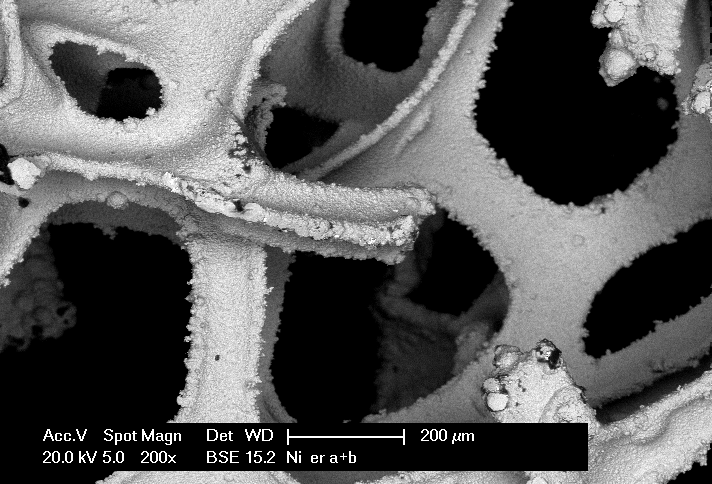
\includegraphics[width = 0.7 \textwidth]{images/ni_er_apb.png}
\end{minipage}
\begin{minipage}[c]{.55\linewidth}
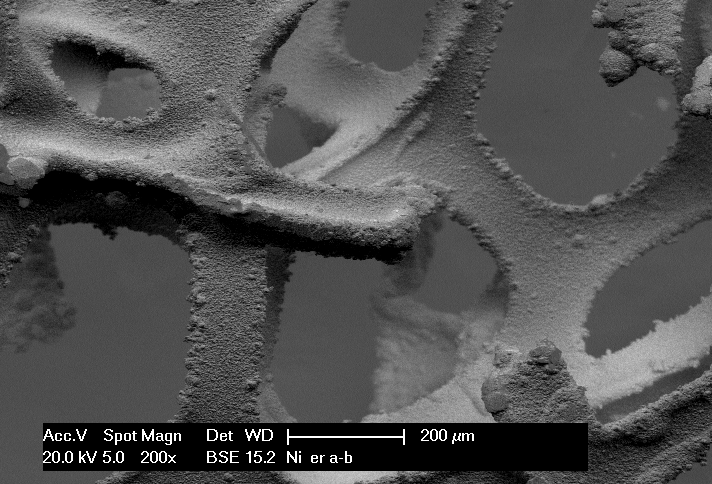
\includegraphics[width = 0.7 \textwidth]{images/ni_er_amb.png}
\end{minipage}
\caption{Observation de l'éponge de nickel utilisant les électrons rétro-diffusés recueillis par le détecteur à semi-conducteur en mode $A+B$ et $A-B$. L'échantillon est ici grossi 200 fois.}
\label{fig:ni_er_apb_amb}
\end{figure}



Le détecteur à semi-conducteur permet également de réaliser un cliché différent en utilisant les mêmes électrons
rétro-diffusés. L'image réalisée avec le mode $A-B$ est présentée sur la figure \ref{fig:ni_er_apb_amb}. Sur ce cliché
le contraste est topographique.


 

\section{Echantillon de silicium}

L'étude, avec les techniques d'imagerie du microscope électronique à balayage, d'un échantillon de silicium permet d'obtenir un grand nombre d'informations.

\subsection{Structure cristallographique de l'échantillon}

On réalise une image de l'échantillon de silicium en collectant les électrons secondaires avec le détecteur d'\ett.
Le cliché obtenu est présenté sur la figure \ref{fig:si_es}. On garde à l'esprit qu'il présente un contraste topographique.
On observe des structures pyramidales en bas-relief ou en haut-relief. Les conditions d'éclairage du cliché ne permettent
pas d'opter pour l'une ou l'autre des solutions (bas-relief ou haut-relief). Ces structures nous informent sur la structure
du matériau et l'observation de ce cliché nous permet de penser que la structure de l'échantillon est cristalline.



\begin{figure}
\centering
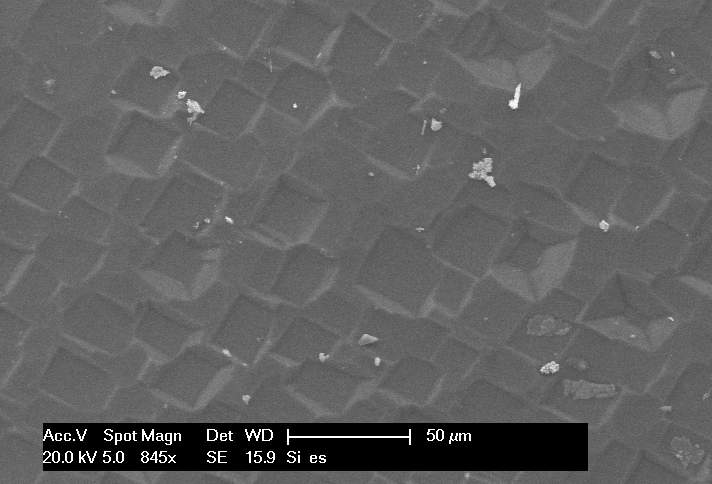
\includegraphics[width=0.7\textwidth]{images/si_es.png}
\caption{Observation d'un échantillon de silicium utilisant les électrons secondaires collectés dans le détecteur d'\ett. L'échantillon est ici grossi 845 fois.}
\label{fig:si_es}
\end{figure}

Afin de déterminer si les pyramides sont en bas-relief ou non on utilise un autre cliché. La figure \ref{fig:si_er_rasant} présente
un cliché réalisé à l'aide du détecteur de \ett mais en collectant les électrons rétrodiffusés. Les électrons utilisés étant rasants,
on observe des effets d'ombre et de lumière. Par exemple une poussière en haut à droite du cliché projette son ombre vers le bas.
On en déduit que l'éclairage provient du haut du cliché. Ainsi il est maintenant possible de se prononcer sur l'enfoncement des pyramides.
Les faces éclairées sont celles situées en bas, ce qui veut dire que les pyramides sont en bas-relief.

\begin{figure}
\centering
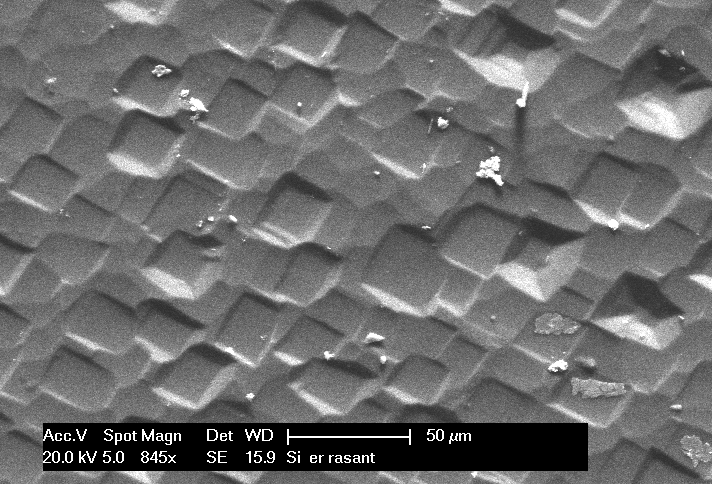
\includegraphics[width=0.7\textwidth]{images/si_er_rasant.png}
\caption{Observation d'un échantillon de silicium utilisant les électrons rétrodiffusés collectés dans le détecteur d'\ett. L'échantillon est ici grossi 845 fois.}
\label{fig:si_er_rasant}
\end{figure}

En utilisant le détecteur à semiconducteur en mode $A+B$, on observe sur la figure \ref{fig:si_er_apb_amb} les contrastes de compositions et en l'occurence qu'il y a deux types de poussières. Mais le plus important pour la détermination de la structure cristallographique est le mode $A-B$. En effet, cela permet de gommer la composition chimique et d'avoir ainsi accès au relief residuel. On observe sur la figure \ref{fig:si_er_apb_amb} donc des carrés ce qui implique une symétrie Pi/2 et donc un axe d'ordre 4. L'orientation du cristal est donc selon le plan (100) ou (010). En effet, une orientation selon le plan (110), on aurait eu un axe d'ordre 3 et donc des formes hexagonales sur le cliché.
\begin{figure}
\begin{minipage}[c]{.55\linewidth}
\centering
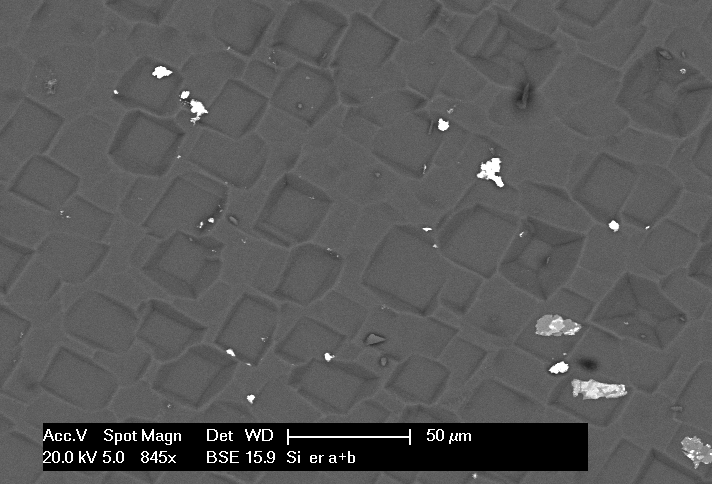
\includegraphics[width=0.7\textwidth]{images/si_er_apb.png}
 \end{minipage}\hfill
\begin{minipage}[c]{.55\linewidth}
\centering
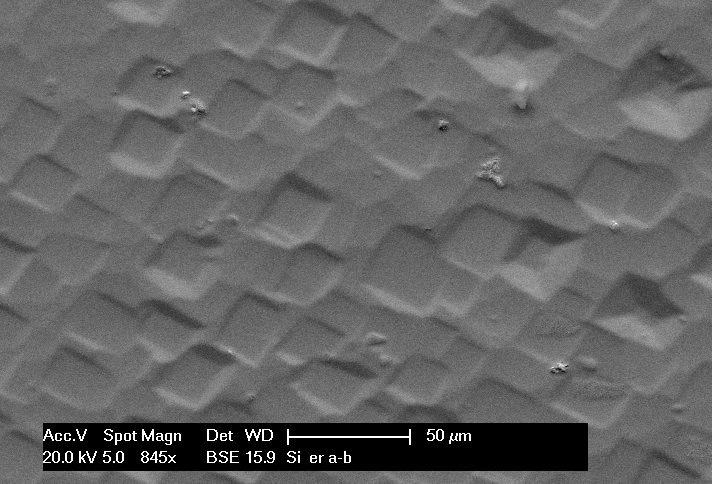
\includegraphics[width=0.7\textwidth]{images/si_er_amb.png}
\end{minipage}
\caption{Observation d'un échantillon de silicium utilisant les électrons rétrodiffusés recueilli par le détecteur semiconducteur en mode $A+B$ et $A-B$. L'échantillon est ici grossi 845 fois.}
\label{fig:si_er_apb_amb}
\end{figure}

\section{Echantillon d'aluminium}
Cette échantillon est la résultante d'un morceau d'aluminium brisé, on peut voir à l'oeil une rugosité importante. Quelles sont les informations que pourra nous donner une étude au microscope MEB.

Avec les électrons secondaire, on voit sur l'échantillon deux types de reliefs. Des déchirures à certains endroit, avec des facettes acérées et des gouffres remplis de boules comme on peut le voir dans la figure \ref{fig:alu_reliefs}. Les deux types de ruptures dans ce même échantillon peuvent être expliqués à l'aide d'un diagramme de phase (figure \ref{fig:diagphase}).
\begin{figure}
\begin{minipage}[c]{.55\linewidth}
\centering
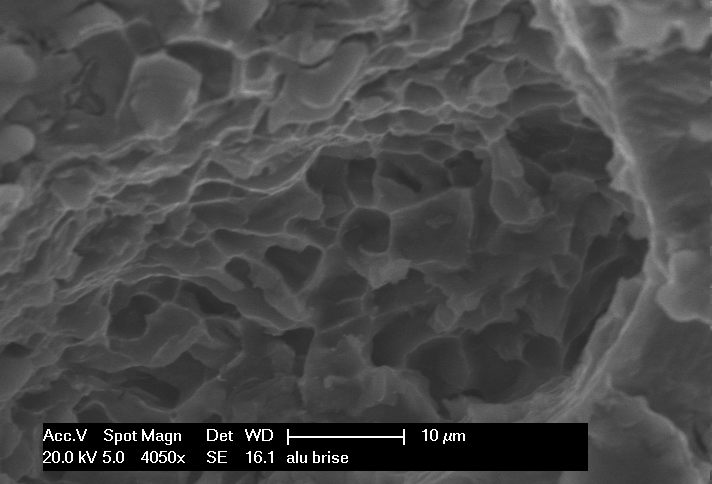
\includegraphics[width=0.7\textwidth]{images/alu_arretes.png}
 \end{minipage}\hfill
\begin{minipage}[c]{.55\linewidth}
\centering
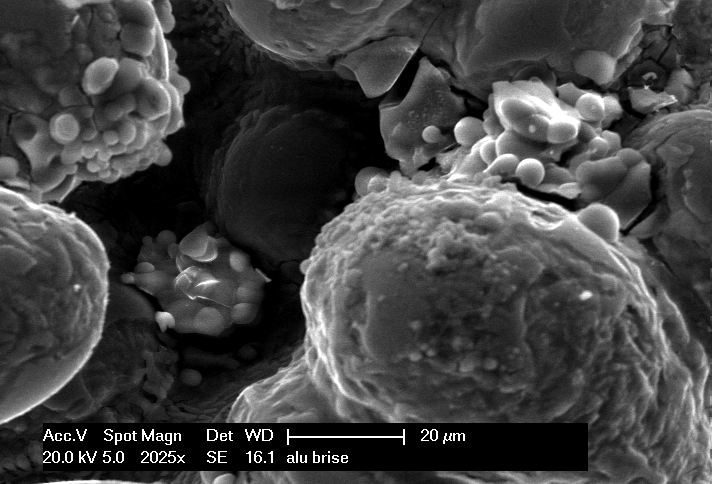
\includegraphics[width=0.7\textwidth]{images/alu_brise.png}
\end{minipage}
\caption{Observation de l'échantillon d'aluminium en utilisant les électrons secondaires}
\label{fig:alu_reliefs}
\end{figure}

\begin{figure}
\centering
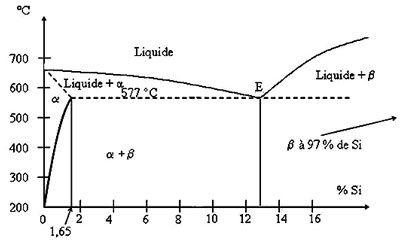
\includegraphics[width=0.7\textwidth]{images/diagphasealusi.jpg}
\caption{diagramme de phase de l'alliage Aluminium Silicium}
\label{fig:diagphase}
\end{figure}

\section*{Conclusion}

On a pu voir lors de ce TP, la large gamme de possibilité offerte par la microscopie MEB. En effet, en tirant partis des différents phénomènes physiques, on peut avoir des informations sur la composition chimique, la répartition des composés dans l'espace, l'état de surface, les plans cristallographiques, le relief de l'échantillon. Ses avantages par rapport à la microscopie optique sont aussi non négligeable, la résolution et la profondeur de champs sont par exemple bien meilleure. Et bien que les échantillons observés doivent être conducteur, on arrive tout de même, par des techniques de déposition à permettre l'obserbation d'échantillons organiques.



\end{document}
